\documentclass[11pt,a4paper]{article}

\usepackage{amsfonts}
\usepackage{amsmath}
\usepackage{geometry}
\usepackage{xcolor}
\usepackage{graphicx}
%\usepackage[subfolder,cleanup]{gnuplottex}
%\usepackage{amsthm}
%\usepackage{enumitem}
%\usepackage{wrapfig}
%\usepackage{subcaption}
%\usepackage{hyperref}
\usepackage{tikz}

\usetikzlibrary{positioning}

\usepackage{enumerate}
\usepackage[shortlabels]{enumitem}
\usepackage{mathrsfs}


\usepackage{lipsum}


% Nicer brackets for operators
\let\originalleft\left
\let\originalright\right
\renewcommand{\left}{\mathopen{}\mathclose\bgroup\originalleft}
\renewcommand{\right}{\aftergroup\egroup\originalright}

% Math operators
\providecommand{\bigO}[1]{\ensuremath{\mathop{}\mathopen{}\mathcal{O}\mathopen{}\left(#1\right)}}

% Macros
\newcommand{\diff}[3][]{\frac{\textrm{d}^{#1}#2}{\textrm{d}{#3}^{#1}}}
\newcommand{\pdiff}[3][]{\frac{\partial^{#1}#2}{\partial{#3}^{#1}}}
\newcommand{\df}{\, \textrm{d}}
%\newcommand{\eps}{\varepsilon}

% Row colouring in tables
%\usepackage[table]{xcolor}
%\rowcolors{2}{gray!25}{white}

% Margin size
\newgeometry{margin=2cm}

% Reference style
%\bibliographystyle{ieeetr}

\title{Optimization Assignment}
\author{Brady Metherall}
\date{16 December 2019}

\begin{document}
\maketitle


\textbf{Problem 1.}
The new system consist of
\begin{align}
    \sum_j^n a_{ij} x_j &\leq b_i, & i &\in M_0, \label{eq:m0} \\
    \sum_j^n (a_{ik} a_{lj} - a_{lk} a_{ij}) x_j, &\leq a_{ik} b_l - a_{lk} b_i & (i,l) &\in M_+ \times M_-. \label{eq:mplus}
\end{align}
The coefficient of $x_k$ in \eqref{eq:m0} and \eqref{eq:mplus} is 0 since $i \in M_0$ and $a_{ik} a_{lk} - a_{lk} a_{ik} = 0$, respectively. Therefore, $x_k$ is not in this new system.

By taking positive linear combinations of the original system we have
\begin{align*}
    a_{ik} \left( \sum_j^n a_{lj} x_j \right) - a_{lk} \left( \sum_j^n a_{ij} x_j \right) \leq a_{ik} \left( b_l \right) - a_{lk} \left( b_i \right),
\end{align*}
because $a_{ik} > 0$ and $-a_{lk} > 0$ since $(i, l) \in M_+^k \times M_-^k$. We can now expand to yield \eqref{eq:mplus}. Note, from the original system we have
\begin{align*}
    \begin{cases}
        \displaystyle a_{ik} x_k \leq b_i - \sum_{j \neq k}^n a_{ij} x_j & i \in M_+^k, \\
        \displaystyle a_{lk} x_k \geq b_l - \sum_{j \neq k}^n a_{lj} x_j & l \in M_-^k. \\
    \end{cases}
\end{align*}
It must then be that
\begin{align*}
    \frac{1}{a_{lk}} \left( b_l - \sum_{j \neq k}^n a_{lj} x_j \right) \leq x_k \leq \frac{1}{a_{ik}} \left( b_i - \sum_{j \neq k}^n a_{ij} x_j \right)
\end{align*}
for all $(i, l) \in M_+^k \times M_-^k$. Therefore,
\begin{align*}
    \max_{l \in M_-^k} \frac{1}{a_{lk}} \left( b_l - \sum_{j \neq k}^n a_{lj} x_j \right) \leq x_k \leq \min_{i \in M_+^k} \frac{1}{a_{ik}} \left( b_i - \sum_{j \neq k}^n a_{ij} x_j \right).
\end{align*}

\textbf{Problem 2.}
\begin{enumerate}[i)]
    \item
    If both systems had a solution, that would imply
    \begin{align*}
        \mathbf{0}^T &= yA, \\
        0 &= (y A) x, \\
        &= y (A x), \\
        &\leq yb, \\
        &< 0,
    \end{align*}
    which is a contradiction. Thus, both systems cannot have solutions.
    \item
    There must exist a $k_*$ such that $d_{k_*} < 0$, otherwise, our new system is in fact consistent.
\end{enumerate}

\textbf{Problem 3.}
\begin{enumerate}[i)]
    \item Both $y_t$ and $z_t$ are binary variables. If production occurs within period $t$, then $y_t = 1$. Furthermore, if production is switched on within period $t$, then $z_t = 1$.
    \item We can express the system in matrix form as
    \begin{align*}
        A
        \begin{pmatrix}
            y \\
            z
        \end{pmatrix}
        \leq
        \begin{pmatrix}
            k \\
            \mathbf{0} \\
            \mathbf{0} \\
            \mathbf{1} \\
            \mathbf{1}
        \end{pmatrix},
    \end{align*}
    where
    \begin{align*}
        A =
        \begin{pmatrix}
            \mathbf{0}^T & \mathbf{1}^T \\
            I - L & -I \\
            -I & I \\
            I & 0 \\
            0 & I
        \end{pmatrix}.
    \end{align*}
    We wish to show that $A$ is totally unimodular, to start, we notice that $A$ is totally unimodular if and only if
    \begin{align*}
        \begin{pmatrix}
            \mathbf{0} & I - L^T & -I \\
            \mathbf{1} & -I & I
        \end{pmatrix}
    \end{align*}
    is totally unimodular, as this is the transpose of $A$ after removing the identity in the lower portion.
\end{enumerate}

\textbf{Problem 4.}
\begin{enumerate}[i)]
    \item The constraint matrix is the vertex-edge incidence matrix, $A$. Therefore, each column contains exactly two 1s. We can then choose the partitions to be $M_1 = V_1$ and $M_2 = V_2$, and the constraint matrix is totally unimodular.
    \item The LP relaxation is
    \begin{align}
        \nonumber \max_x & \sum_{e \in E} x_e, \\
        \text{s.t.} \quad A x &\leq 1, \label{eq:edges} \\
        \nonumber x_e &\geq 0.
    \end{align}
    The dual is then given by
    \begin{align}
        \nonumber \min_y & \sum_{v \in V} y_v, \\
        \text{s.t} \quad A^T y &\geq 1, \label{eq:nodes} \\
        \nonumber y_v &\geq 0.
    \end{align}
    Since $A^T$ is totally unimodular as well, the solution to the LP is identical to the IP. Additionally, for the minimum cardinality node covering, we do not require $y_v$ to be greater than one, and so $y_v \in \{ 0, 1 \}$.
    \item We can find trivial feasible solutions to \eqref{eq:edges} and \eqref{eq:nodes} is the empty matching and the full graph. Then by the Strong Duality Theorem and since $A$ is totally unimodular, K\"{o}nig's Theorem holds.
\end{enumerate}

\textbf{Problem 5.}
\begin{enumerate}[i)]
    \item The LP relaxation of the binary knapsack problem is
    \begin{gather}
        \max_x \, c^T x, \\
        \text{s.t.} \quad
        \begin{pmatrix}
            a^T \\
            I
        \end{pmatrix}
        x \leq
        \begin{pmatrix}
            b \\
            \mathbf{1}
        \end{pmatrix}.
        \label{eq:ks}
    \end{gather}
    With associated dual
    \begin{gather*}
        \max_y \, (b, \ \mathbf{1}^T) y, \\
        \text{s.t.} \quad
        \begin{pmatrix}
            a & I
        \end{pmatrix}
        y \geq c.
    \end{gather*}
    We find that \eqref{eq:ks} is an equality for the first $r$ rows. Expanding the constraint yields
    \begin{align}
        a_i y_1 + y_{i+1} \geq c_i.
        \label{eq:ksdual}
    \end{align}
    Now, by complementary slackness, \eqref{eq:ksdual} must be active for $i \leq r$, and $y_i = 0$ for $i = r + 1, \cdots, n + 1$. Evaluating \eqref{eq:ksdual} at $i = r$ gives
    \begin{align*}
        y_1 = \frac{c_r}{a_r},
    \end{align*}
    and so,
    \begin{align*}
        y_{i+1} = c_i - a_i \frac{c_r}{a_r}.
    \end{align*}
    We can now show that the claimed solution is indeed optimal by showing the values of the objective functions are equal:
    \begin{align*}
        (b, \ \mathbf{1}^T) y &= b \frac{c_r}{a_r} + \sum_j^{r-1} \left( c_j - a_j \frac{c_r}{a_r} \right), \\
        &= b \frac{c_r}{a_r} + \sum_j^{r-1} c_j - \frac{c_r}{a_r} \sum_j^{r-1} a_j, \\
        &= \frac{c_r}{a_r} \left( b - \sum_j^{r-1} a_j \right) + \sum_j^{r-1} c_j, \\
        &= \sum_j^{r-1} c_j + c_r \frac{b - \sum_j^{r-1} a_j}{a_r}, \\
        &= c^T x.
    \end{align*}
    In the case that $x_r = 0$, our analysis remains the same, and the claimed solution is still optimal.
    \item
    \begin{figure}[tbp]
        \centering
        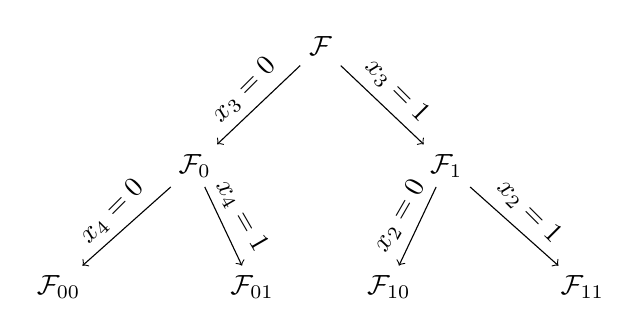
\begin{tikzpicture}
            \node [rectangle] (A) {$\mathcal{F}$};

            \node (B) [below left=of A] {$\mathcal{F}_0$};
            \node (C) [below right=of A] {$\mathcal{F}_1$};

            \node (D) [below left=of B] {$\mathcal{F}_{00}$};
            \node (E) [below right=of B, xshift=-10mm] {$\mathcal{F}_{01}$};

            \node (F) [below left=of C, xshift=10mm] {$\mathcal{F}_{10}$};
            \node (G) [below right=of C] {$\mathcal{F}_{11}$};


            \draw [->] (A) to node [rotate=45, anchor=south] {$x_3 = 0$} (B);
            \draw [->] (A) to node [rotate=-45, anchor=south] {$x_3 = 1$} (C);

            \draw [->] (B) to node [rotate=45, anchor=south] {$x_4 = 0$} (D);
            \draw [->] (B) to node [rotate=-60, anchor=south] {$x_4 = 1$} (E);

            \draw [->] (C) to node [rotate=60, anchor=south] {$x_2 = 0$} (F);
            \draw [->] (C) to node [rotate=-45, anchor=south] {$x_2 = 1$} (G);
        \end{tikzpicture}
        \caption{Binary tree of branch and bound.}
        \label{fig:bnb}
    \end{figure}
    We seek the solution to
    \begin{gather*}
        \max_x \, (17, \, 10, \, 25, \, 17) x, \\
        \text{s.t.} \quad (5, \, 3, \, 8, \, 7) x \leq 12, \\
        x \in \mathbb{Z}_2^4,
    \end{gather*}
    using branch and bound, as depicted in Figure \ref{fig:bnb}. As the system is well ordered already, we may use the result of the previous question to find the relaxed greedy solution $(1, \, 1, \, 1/2, \, 0)^T$. This gives us the upper bound $\bar{z} = \lfloor 39.5 \rfloor$, lower bound $\underbar{$z$} = 27$, and incumbent $(1, \, 1, \, 0, \, 0)^T$. As $x_3 \in \mathbb{Q}$, we branch $\mathcal{F}$ into $\mathcal{F}_0$ with $x_3 = 0$, and $\mathcal{F}_1$ with $x_3 = 1$.

    Considering first $\mathcal{F}_1$, as we wish to maximize, we find the simplified problem
    \begin{gather*}
        \max_x \, (17, \, 10, \, 17)
        \begin{pmatrix}
            x_1 \\
            x_2 \\
            x_4
        \end{pmatrix}, \\
        \text{s.t.} \quad (5, \, 3, \, 7)
        \begin{pmatrix}
            x_1 \\
            x_2 \\
            x_4
        \end{pmatrix}
        \leq 4.
    \end{gather*}
    Clearly, from the constraints $x_1 = 0$ and $x_4 = 0$ as they must be integers. This allows us to branch into $\mathcal{F}_{10}$ and $\mathcal{F}_{11}$ for $x_2 = 0$ and $x_2 = 1$, respectively. The node $\mathcal{F}_{10}$ contains a single feasible point which yields 25 as the objective, as this is less than $\underbar{$z$}$, and therefore, may be pruned. Similarly, $\mathcal{F}_{11}$ gives the improved lower bound $\underbar{z} = 35$ with incumbent .

    Moving back to $\mathcal{F}_{0}$, we have the problem
    \begin{gather*}
        \max_x \, (17, \, 10, \, 17)
        \begin{pmatrix}
            x_1 \\
            x_2 \\
            x_4
        \end{pmatrix}, \\
        \text{s.t.} \quad (5, \, 3, \, 7)
        \begin{pmatrix}
            x_1 \\
            x_2 \\
            x_4
        \end{pmatrix}
        \leq 12.
    \end{gather*}
    Solving the LP relaxation we find $(1, \, 1, \, 0, \, 4/7)^T$, and so we branch to $\mathcal{F}_{00}$ and $\mathcal{F}_{00}$ based on the value of $x_4$. In the case $x_4 = 0$ ($\mathcal{F}_{00}$), we find $(1, \, 1, \, 0, \, 0)^T$, which is a former incumbent, and can be pruned. On the other hand, $x_4 = 1$ and $\mathcal{F}_{01}$, we find $(1, \, 0, \, 0, \, 1)^T$ which produces an objective of 34. This branch may also be pruned as this is worse than our current incumbent.

    Now all of the branches have been exhausted, and therefore, we have found the optimal solution of $(0, \, 1, \, 1, \, 0)^T$.
\end{enumerate}

\textbf{Problem 6.}

\begin{enumerate}[i)]
    \item We can show that $w \geq z$ since
    \begin{align*}
        w &\geq g(x) & \forall x &\in \mathscr{R}, \\
        &\geq g(x) & \forall x &\in \mathscr{F}, \\
        &\geq c^T x & \forall x &\in \mathscr{F}, \\
        &\geq z.
    \end{align*}
    \item We can simplify the objective function in (GR) by
    \begin{align*}
        \frac{c_k}{a_k} b + \max_x \sum_{j \ne k} \left( c_j - \frac{c_k}{a_k} a_j \right) x_j &=
            \max_x \left( \frac{c_k}{a_k} b + \sum_{j \ne k} c_j x_j + c_k x_k - c_k x_j - \frac{c_k}{a_k} \sum_{j \ne k} a_j x_j \right), \\
        &= \max_x \left( \frac{c_k}{a_k} \sum_j a_j x_j + \sum_j c_j x_j - c_k \left( \sum_{j \ne k} \frac{a_j}{a_k} x_j + \frac{a_k}{a_k} x_k \right) \right), \\
        &= \max_x \left( \frac{c_k}{a_k} \sum_j a_j x_j + \sum_j c_j x_j - c_k \sum_j \frac{a_j}{a_k} x_j \right), \\
        &= \max_x c^T x,
    \end{align*}
    to show that it is equivalent to the objective in (EKP). Additionally, any feasible solution to (EKP) must also be a feasible solution to (GR):
    \begin{align*}
        0 &= \sum_j a_j x_j - b, \\
        &= \sum_{j \ne k} a_j x_j + a_k x_k - b, \\
        &\equiv \sum_{j \ne k} a_j x_j - b \, \text{(mod $a_k$)},
    \end{align*}
    since $x \in \mathbb{Z}^n$.
    \item this is part 3 right


    \begin{figure}[tbp]
        \centering
        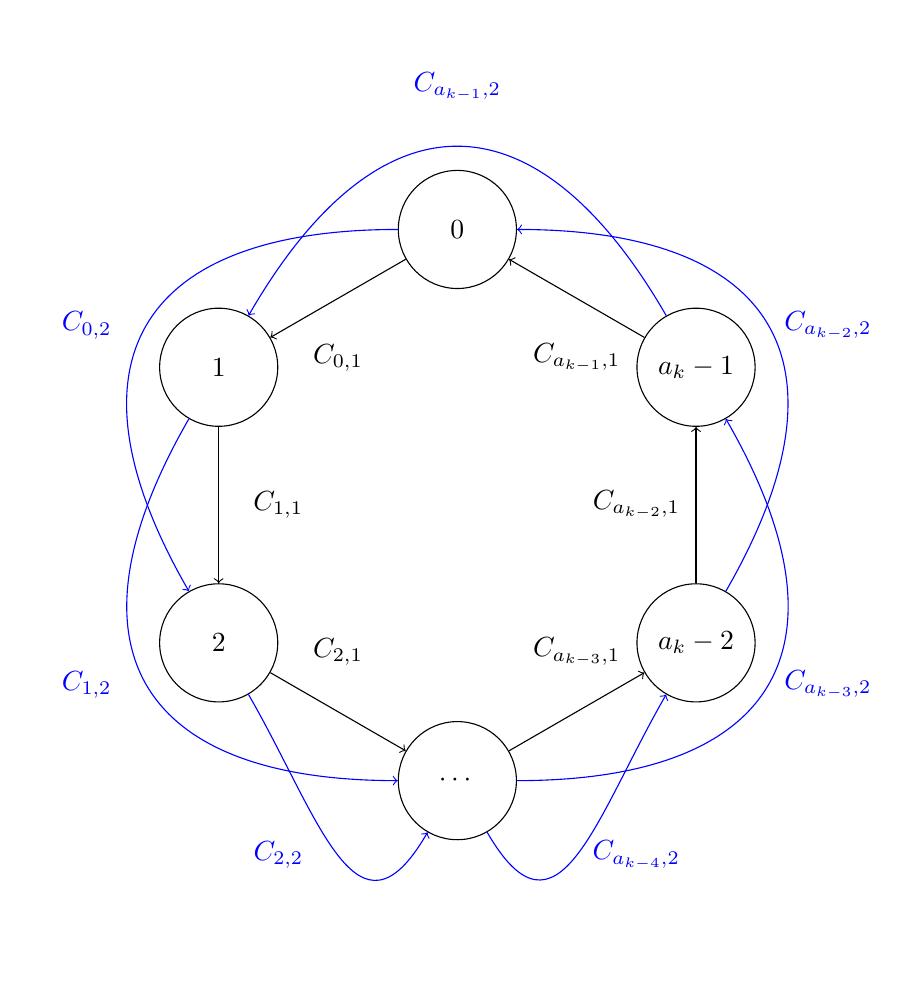
\begin{tikzpicture}[minimum size=1.5cm]
            \def \radius {3.5cm}

            % Nodes
            \node (A) [draw, circle] at ({60 * 0 + 90}:\radius) {$0$};
            \node (B) [draw, circle] at ({60 * 1 + 90}:\radius) {$1$};
            \node (C) [draw, circle] at ({60 * 2 + 90}:\radius) {$2$};
            \node (D) [draw, circle] at ({60 * 3 + 90}:\radius) {$\cdots$};
            \node (E) [draw, circle] at ({60 * 4 + 90}:\radius) {$a_k - 2$};
            \node (F) [draw, circle] at ({60 * 5 + 90}:\radius) {$a_k - 1$};
            % Length 1 edges
            \draw [->] (A) to node [anchor=north] {$C_{0,1}$} (B);
            \draw [->] (B) to node [anchor=west] {$C_{1,1}$} (C);
            \draw [->] (C) to node [anchor=south] {$C_{2,1}$} (D);
            \draw [->] (D) to node [anchor=south] {$C_{a_{k-3},1}$} (E);
            \draw [->] (E) to node [anchor=east] {$C_{a_{k-2},1}$} (F);
            \draw [->] (F) to node [anchor=north] {$C_{a_{k-1},1}$} (A);
            % Length 2 edges
            \draw [->, blue] (A) to [out=180, in=120, looseness=1.6, blue] node [anchor=east] {$C_{0,2}$} (C);
            \draw [->, blue] (B) to [out=240, in=180, looseness=1.6, blue] node [anchor=east] {$C_{1,2}$} (D);
            \draw [->, blue] (C) to [out=300, in=240, looseness=1.6, blue] node [anchor=east] {$C_{2,2}$} (D);
            \draw [->, blue] (D) to [out=300, in=240, looseness=1.6, blue] node [anchor=west] {$C_{a_{k-4},2}$} (E);
            \draw [->, blue] (D) to [out=0, in=300, looseness=1.6, blue] node [anchor=west] {$C_{a_{k-3},2}$} (F);
            \draw [->, blue] (E) to [out=60, in=0, looseness=1.6, blue] node [anchor=west] {$C_{a_{k-2},2}$} (A);
            \draw [->, blue] (F) to [out=120, in=60, looseness=1.6, blue] node [anchor=south] {$C_{a_{k-1},2}$} (B);
        \end{tikzpicture}
        \caption{System (GR) depicted as a shortest path problem.}
        \label{fig:shortpath}
    \end{figure}
\end{enumerate}

\textbf{Problem 7.}
By assumption
\begin{align*}
    a^T x^* &= \sum_{j \in \{ i : x_i^* = 1 \}} a_j, \\
    &> r.
\end{align*}
Therefore, there exists a cover, $C$, such that
\begin{align*}
    \sum_{j \in C} a_j x_j \leq r
\end{align*}
is a cut for $x^*$. Since the algorithm first reorders $a_j$ to be in descending order, it must be that it finds the minimal cover.

\textbf{Problem 8.}
Consider the system
\begin{align*}
    \min_x \, &\mathbf{1}^T x \\
    \text{such that }
    \begin{pmatrix}
        6 & 1 \\
        -3 & 0 \\
        -1 & 0 \\
        0 & -1
    \end{pmatrix}
    x &\leq
    \begin{pmatrix}
        4 \\
        -1 \\
        0 \\
        0
    \end{pmatrix}.
\end{align*}
By examining the first two rows, we find that
\begin{align*}
    1 &\leq 3 x_1, \\
    2 &\leq 6 x_1, \\
    2 \leq 6 x_1 &\leq 6 x_1 + x_2 \leq 4.
\end{align*}
We can then simplify this to show
\begin{align*}
    2 \leq 6 x_1 \leq 4, \\
    \frac{1}{3} \leq x_1 \leq \frac{2}{3}
\end{align*}
which has no feasible solutions for $x_1 \in \mathbb{Z}$, and therefore the IP is infeasible.

\textbf{Problem 9.}

\begin{enumerate}[i)]
    \item Take the cover, $C_i$, to be $\{ j : 1 \leq j \leq n \}$. Then, by assumption,
    \begin{align*}
        \sum_j c_{ij} > b_i,
    \end{align*}
    therefore, for $x$ to be feasible there must be at least one $0$ entry. Thus,
    \begin{align*}
        \sum_j x_{ij} &\leq n - 1, \\
        &\leq |C_i| - 1,
    \end{align*}
    as desired.
    \item If $x_{mj^*}^* > 1/2$ then GUB is not a good branching rule. As $\sum_i x_{ij} = 1$, then $p = m$. Thus, $\mathscr{F}_1 = \emptyset$ and $\mathscr{F}_2 = \mathscr{F}$. A better rule is follows:
    \begin{itemize}
        \item Reorder the elements such that $\tilde{x}_{i,j^*} \leq \tilde{x}_{i+1,j^*}$.
        \item Reorder the elements once again such that (without loss of generality)
        \begin{align*}
            \tilde{x}_{1,j^*}, \tilde{x}_{3,j^*}, \cdots, \tilde{x}_{m,j^*}, \tilde{x}_{(m - 1),j^*}, \tilde{x}_{(m - 3),j^*}, \cdots, \tilde{x}_{2,j^*}.
        \end{align*}
        \item Apply GUB on this new arrangement.
    \end{itemize}
\end{enumerate}

%\bibliography{Ref}

\end{document}
